\PassOptionsToPackage{utf8}{inputenc}
\documentclass{bioinfo}
\copyrightyear{2020} \pubyear{2020}

\access{Advance Access Publication Date: Day Month Year}
\appnotes{Manuscript Category}

\usepackage{longtable}
\usepackage{comment}
\usepackage{colortbl}
\usepackage[table]{xcolor}
\usepackage{float}
\usepackage{booktabs}
\usepackage{lipsum}
\usepackage{multirow}
\usepackage{graphicx,paralist}
\usepackage[document]{ragged2e}
\usepackage{amsthm}
\usepackage{amsmath}
\usepackage{setspace}
\usepackage[draft]{hyperref}
\usepackage{fixltx2e}
\usepackage{natbib}
%\usepackage[font=bf]{caption}
\usepackage{multicol}

\def\CorShrink{\texttt{CorShrink}}
\def\CorShrinkk{\texttt{CorShrink2}}
\def\Robocov{\texttt{Robocov}}
\def\Robospan{\texttt{Robospan}}
\def\pRobospan{\texttt{pRobospan}}
\def\Corspan{\texttt{Corspan}}



\begin{document}
\firstpage{1}

\subtitle{Subject Section}

\title[a]{A convex optimization framework for gene-level tissue network estimation with missing data and its application in disease architecture}
\author[Dey \& Mazumder.]{Kushal K. Dey \,$^{\text{\sfb 1,}*}$, Rahul Mazumder \,$^{\text{\sfb 2, }*}$}
\address{$^{\text{\sf 1}}$Department of Epidemiology, Harvard T. H. Chan School of Public Health, Boston, MA \\
$^{\text{\sf 2}}$Sloan School of Management, Operations Research Center and Center for Statistics, MIT, Cambridge, MA.}

\corresp{$^\ast$ denotes authors to whom correspondence should be addressed.}

\history{Received on XXXXX; revised on XXXXX; accepted on XXXXX}

\editor{Associate Editor: XXXXXXX}

 
\abstract{\textbf{Motivation:} \justifying Genes with correlated expression across individuals in multiple tissues are potentially informative for systemic genetic activity spanning these tissues. In this context, the tissue-level gene expression data across multiple subjects from the Genotype Tissue Expression (GTEx) Project is a valuable analytical resource. Unfortunately, the GTEx data is fraught with missing entries owing to subjects often contributing only a subset of tissues. In such a scenario, standard techniques of correlation matrix estimation with or without data imputation do not perform well. To solve this problem, we propose \Robocov{}, a novel convex optimization-based framework for robustly learning sparse covariance or inverse covariance matrices for missing data problems. \\
\textbf{Results:} \Robocov{} produces more interpretable visual representation of correlation and causal structure in simulation settings and GTEx data analysis. We also show that \Robocov{} estimators have a lower false positive rate than competing approaches for missing data problems.  Genes prioritized by the average value of \Robocov{} correlations or partial correlations across tissues are enriched for pathways related to systemic activities such as signaling pathways, circadian clock and immune function. SNPs linked to these prioritized genes showed high enrichment and unique information for blood-related traits; in comparison, no disease signal is observed for SNPs characterized analogously using standard correlation estimator.\\
\textbf{Availability:} \Robocov{} is available as an R package \url{https://github.com/kkdey/Robocov}. \\
\textbf{Contact:} \href{kdey@hsph.harvard.edu}{kdey@hsph.harvard.edu}\\
\textbf{Supplementary information:} Supplementary data are available at \textit{Bioinformatics} online.}
\maketitle

\justifying
\section{Introduction}

The gene expression data from nearly 50 tissues across more than 500 post-mortem donor individuals from Genotype Tissue Expression (GTEx) project has proved to be a valuable resource for understanding tissue-specific and tissue-shared genetic architecture~\cite{gtex2015, gtex2017, dey2017, aguet2019}. Here we are interested in one specific aspect of tissue-shared gene regulation: the correlation and partial correlation in gene expression for  different tissue pairs based on individual donor level data.  A major challenge in this context is the extensive amount of missing entries in gene expression data---each donor contributes only a subset of tissues for sequencing. 
Common imputation based methods do not work well here as reported in~\cite{dey2019}, owing to stringent assumptions about missing entries being close to some central tendency (median) or adhering to some low-dimensional representation of the observed entries~\cite{mazumder2010spectral,mazumder2015}. Popular shrinkage and/or sparse correlation or partial correlation estimators such as \textit{corpcor}~\cite{ledoit2003improved, schafer2005shrinkage}, GLASSO~\cite{friedman2008} or CLIME~\cite{cai2011} are not designed for data with missing values. 

A recently proposed approach, \CorShrink{}~\cite{dey2019}, co-authored by one of the authors of this paper (Dey), accounts for missing data through adaptive shrinkage~\cite{stephens2016} of correlations. \CorShrink{} does not guarantee a positive semidefinite (PSD) matrix as part of its EM-based framework, and necessitates a post-hoc modification to ensure a PSD correlation matrix. Furthermore, \CorShrink{} does not extend to conditional graph or partial correlation estimation. Here, we propose a new approach based on convex optimization: \Robocov{} that applies to both covariance and inverse covariance matrix estimation in the presence of missing data under the following regularization principles:
(a) the covariance matrix is sparse (i.e., has a few nonzero entries) or (b) the inverse covariance matrix is sparse. 

\Robocov{} does not \emph{impute} missing values per-se\footnote{Expectation Maximization (EM)~\cite{Dempster1977} methods typically used for estimation with missing values depend upon probabilistic modeling assumptions and lead to highly nonconvex problems
posing computational challenges.}---it directly estimates the covariance or inverse covariance matrices in the presence of missing values. To handle missing values, we consider a loss function that depends upon the pairwise covariance terms (computed based on the observed samples) but incorporates an adjustment to guard against our lack of knowledge regarding the missing observations. For inverse covariance estimation, \Robocov{} uses a robust optimization based approach~\cite{ben2009robust,bertsimas2011theory} that accounts for the uncertainty in estimating the pairwise sample covariance terms (due to the presence of missing values). Interestingly, both lead to convex optimization formulations that are amenable to modern optimization techniques~\cite{BV2004}---they are scalable to moderate-large scale instances; and unlike conventional EM methods (that lead to nonconvex optimization tasks), our estimators attain the global solution of the optimization formulations defining the 
\Robocov{} estimators. 

Our experiments suggest that \Robocov{} estimators for correlation and partial correlation matrices have lower false positive rate compared to competing approaches for missing data problems.  When applied to the GTEx gene expression data with~$\sim70\%$ missing data, \Robocov{} produced less cluttered and highly interpretable visualization of correlation and conditional graph architecture. From a biological perspective, a gene with high correlation in expression across many tissue pairs is potentially reflective of more systemic biological processes spanning multiple tissues. To this end, we prioritized genes based on the average \Robocov{} estimated correlation (partial correlation) across all tissue-pairs; we call them  \Robospan{} (\pRobospan{}) genes. A pathway enrichment analysis of  \Robospan{} (\pRobospan{}) genes showed enrichment in systemic functional pathways and the immune system.  SNPs linked to \Robospan{} (\pRobospan{}) genes were tested for autoimmune disease informativeness by applying Stratified LD-score regression (S-LDSC) to 11 common blood-related traits (5 autoimmune diseases and 6 blood cell traits; average $N$=306K), conditional on a broad set of  annotations. \Robospan{} and \pRobospan{} genes showed high disease informativeness for blood-related traits. In comparison, \Corspan{} genes defined similarly using the standard correlation estimator were non-informative. This highlights the biological and disease-level significance of our work.




\section{Methods}\label{sec:methods-materials}

Let $X_{N \times P}$ be a data matrix with $N$ samples and $P$ features, where some of the entries $X_{np}$ may be missing, denoted here by $\text{NA}$. Let $X^f$ denote the fully-observed version of the partially-observed data matrix\footnote{Note that  $X$ is a restriction of $X^f$ to the observed entries.} $X$. We assume that samples are independent and follow a Multivariate Normal distribution: i.e., 
$X^f_{n,*} \sim \text{MVN} ( 0, \Sigma )$ 
%\begin{equation}\label{eq:normal_dist}
%    X^f_{n,*} \sim \text{MVN} ( 0, \Sigma ) ~~~\text{and}~~~\Omega = \Sigma^{-1}
%\end{equation}
where $\Sigma_{P \times P}$ and $\Omega:=\Sigma^{-1}$ (also of size $P \times P$) denote the model covariance and inverse covariance matrices respectively. 
Based on the observed entries, we obtain a matrix $\hat{\Sigma}$ of pairwise covariances such that for all $i, j \in \{1, \ldots, P\}$:
\begin{equation}\label{eq:standard_cov}
   \hat{\Sigma}_{ij} := \frac{1}{n_{ij} - 1} \sum_{n: X_{ni} \neq \text{NA}, X_{nj} \neq \text{NA}} (X_{ni} - \bar{X}_{i})(X_{nj} - \bar{X}_{j})
\end{equation}
where, $\bar{X}_{k}$ denotes the sample mean of feature $k$ based on the observed entries; and $n_{ij}$ is the number of samples $n$ with non-missing entries in both features $i$ and $j$. Let $n_i$ denote the number of observed samples (i.e., not missing) for feature $i$. For our analysis, we will assume\footnote{If necessary, as a pre-processing step, we remove features so that the condition $n_{ij}>2$ is satisfied for all $i,j$.} that $n_{ij}>2$ for all $i,j$.
We note that the matrix of all pairwise covariance terms: $\hat{\Sigma} = ((\hat{\Sigma}_{ij}))$, as defined in~\eqref{eq:standard_cov}, need not be positive semidefinite due to the presence of missing values in the data matrix.

 \subsection{Robocov covariance estimator}\label{sec:cov-estimator}

%The general optimization framework for \Robocov{} covariance estimator is a regularized criterion of the form: 
%\begin{equation}\label{eq:opt1-general-RM}
% \begin{aligned}
% & \text{min} 
%    &&  \mathcal{L} (\Sigma) + \lambda \xi (\Sigma)
% \end{aligned}
% \end{equation}
% where $\mathcal{L}(\Sigma)$ is the data fidelity term and $\xi(\Sigma)$ is the regularizer (or penalty function) encoding our prior beliefs about the estimator $\Sigma$.
%$\xi(\Sigma)$ represent the  data fidelity function and the penalty function respectively. 
%We present different estimators that are instances of Problem~\eqref{eq:opt1-general-RM} --- they depend upon different choices of the loss function and the regularizer. 

We first present the \Robocov{} covariance matrix estimator---this leads to an estimate of $\Sigma$ via the following regularized criterion: 
\begin{equation}\label{eq:opt1-RM}
 %%\begin{aligned}
    \text{min} ~ \sum_{i<j} |\Sigma_{ij}|~~
    ~~\text{s.t.}~~~~\Sigma \succeq 0,~~
   % &&& \hat{\Sigma} = \text{pairwise sample covariance} \\
   | \hat{\Sigma}_{ij} - \Sigma_{ij} |  \leq  C_{ij},  ~\forall i,j
%% \end{aligned}
\end{equation}
where $\Sigma$ is the optimization variable and $C_{ij}$s are data-driven constants that control the amount by which $\Sigma_{ij}$ can differ from the sample version $\hat{\Sigma}_{ij}$. Problem~\eqref{eq:opt1-RM} minimizes a convex penalty function (this encourages sparsity~\cite{hastie2015statistical} in $\Sigma_{ij}$s) subject to convex constraints (note that $\Sigma$ is positive-semidefinite i.e., $\Sigma \succeq 0$). Problem~\eqref{eq:opt1-RM} is a convex semidefinite optimization problem~\cite{BV2004}; and can be solved efficiently by modern semidefinite optimization algorithms for moderately large instances (e.g, $P \sim 1000$) using (for example) the SCS solver in CVX software~\cite{BV2004,o2016conic,Boyd2004, Fu2017}.


%Note that Problem~\eqref{eq:opt1-RM} minimizes a convex penalty function subject to convex constraints --- the optimization variable $\Sigma$ is positive-semidefinite (denoted as $\Sigma \succeq 0$). Hence~\eqref{eq:opt1-RM} is a convex semidefinite optimization problem~\cite{BV2004}; and can be solved efficiently by modern semidefinite optimization algorithms for moderately large instances (e.g, $P \sim 1000$) using (for example) the SCS solver in CVX software \cite{BV2004,o2016conic,Boyd2004, Fu2017}.
%\textcolor{red}{(basically, we can solve this in CVXR; or we can use SCS solver to solve p = 1000-ish problems)---not sure where to write this. At least we should cite some papers here. Some papers are~\cite{o2016conic,BV2004}.} 
%%%$\hat{\Sigma}$ is the pairwise covariance matrix~\eqref{eq:standard_cov}, and %%$\Sigma \succeq 0$ denotes that $\Sigma$ is positive-semi-definite. 
%The objective function in~\eqref{eq:opt1-RM} minimizes the $\ell_{1}$-norm on the entries of $\Sigma$; and induces sparsity in the solution \cite{hastie2015statistical}. 
%sparsity on the solution and the penalty function imposes 
%The constraint $|\hat{\Sigma}_{ij} - \Sigma_{ij}| \leq C_{ij}$ for all $i,j$
%is the data-fidelity term --- it constrains the entries of the estimated covariance matrix (i.e., $\Sigma_{ij}$) to be close to the sample covariance $\hat{\Sigma}_{ij}$---that is, 
%$\Sigma_{ij} \in [\hat{\Sigma}_{ij} - C_{ij}, \hat{\Sigma}_{ij} + C_{ij}]$. Here, $C_{ij}$ controls the amount by which $\Sigma_{ij}$ can differ from 
%the sample version $\hat{\Sigma}_{ij}$. 




We compute $C_{ij}$ based on the Fisher's Z-Score~\cite{fisher1915, fisher1921} (for a complete derivation see Supplementary Note):
\begin{equation}\label{eq:defineC}
\begin{aligned}
    C_{ij} & = \hat{\sigma}_{i} \hat{\sigma}_{j} \min \left (2,  \eta (n_{ij})  \left \{ 3 (1 - \hat{R}^2_{ij}) + 2 \sqrt{3} \eta (n_{ij}) \right \} \right )
    %\\
    %& \eta(n_{ij})  = \sqrt{\frac{1}{n_{ij} - 1} + \frac{2}{(n_{ij} - 1)^2}}
\end{aligned}
\end{equation}
where  $\eta(n_{ij})  = \sqrt{{1}/{(n_{ij} - 1)} + {2}/{(n_{ij} - 1)^2}}$;
and $\hat{R}$ is the pairwise sample correlation matrix derived from $\hat{\Sigma}$

In summary, we note that our proposed \Robocov{} estimator does not impute missing values per-se --- it directly leads to an estimate for the covariance matrix $\Sigma$ while taking into  account the presence of missing-values in the data matrix.  

%We also explore some other choices of the loss function $\mathcal{L}$ that lead to similar results on real data. 

While~\eqref{eq:opt1-RM} leads to a covariance matrix estimator, this can be modified to deliver a correlation matrix instead of a covariance matrix: 
\begin{equation}\label{eq:opt1-RM-R}
 \begin{aligned}
    \text{min} ~~~& \sum_{i<j} |\mathcal{R}_{ij}| \\
    \text{s.t.}~~~& ~\mathcal{R} \succeq 0, \mathcal{R}_{ii} = 1, \forall i, ~~~ | \hat{R}_{ij} - \mathcal{R}_{ij} |  \leq  C^{(R)}_{ij}, ~\forall i,j
 \end{aligned}
\end{equation}
where $\mathcal{R}$ is the optimization variable and $C^{(R)}_{ij} = \frac{\hat{C}_{ij}}{\hat{\sigma}_{i} \hat{\sigma}_{j}}$. See the Supplementary Note for additional details. 

In the Supplementary Note, we present a  
framework given by the minimization of a regularized loss function that generalizes the 
estimator presented in~\eqref{eq:opt1-RM}. 
%%In practice, we found that many of these estimators lead to similar results on real %%datasets---therefore, in this paper, we focus our attention on the basic %%estimator~\eqref{eq:opt1-RM}. 

\subsection{Robocov inverse covariance estimator}\label{sec:invcov-estimator}
We present a regularized likelihood framework to estimate the inverse covariance matrix ($\Omega$) under a sparsity constraint.
%and subsequently obtain a partial correlation matrix. 
%%We use a regularized likelihood framework to estimate $\Omega$ under a %%sparsity constraint. An appealing aspect of our estimator is that 
Our optimization criterion is 
convex in $\Omega$ (and not $\Sigma$ which was the case in Section~\ref{sec:cov-estimator}).


Recall that GLASSO minimizes an $\ell_{1}$-norm regularized negative log-likelihood criterion (fully observed case); and is given by:
\begin{equation}\label{glasso-problem-1}
\min_{\Omega \succ 0}~~~ -\log\det(\Omega) + \langle \tilde{\Sigma}, \Omega \rangle + \lambda \sum_{ij} |\Omega_{ij}|
\end{equation}
where, $L(\Omega; \tilde{\Sigma}):=-\log\det(\Omega) + \langle \tilde{\Sigma}, \Omega \rangle$ is the negative log-likelihood (ignoring irrelevant constants), $\tilde{\Sigma}$ is the fully observed sample covariance matrix and $\lambda \geq 0$ is the regularization parameter. 
Replacing $\tilde{\Sigma}$ by the observed matrix $\hat{\Sigma}$ in~\eqref{glasso-problem-1} is problematic 
due to the error in estimating the pairwise covariances arising from the
missing values (different cell entries of the sample covariance matrix involve different effective sample sizes $n_{ij}$s leading to varying accuracies in estimating $\tilde{\Sigma}_{ij}$s). To account for this uncertainty, we use ideas from robust optimization~\cite{ben2009robust,bertsimas2011theory}---to the best of our knowledge, this approach has not been used earlier in the context of sparse inverse covariance estimation (in the presence of missing values).
%for the missing values by using polyhedral uncertainty sets for sparse $\Omega$ estimation; to the best of our knowledge, such an approach has not been attempted before. 
Our robust optimization approach minimizes the worst-case loss arising from the errors in estimating the cell entries $\tilde{\Sigma}_{ij}$s. This leads to a min-max optimization problem of the form:
\begin{equation}\label{eq:opt2-RM}
    \min_{\Omega \succeq 0} ~ \max_{\substack{\Delta \\ 
    |\Delta_{ij}| \leq D_{ij}, \forall i,j}}~ 
    \left \{ -\log \det( \Omega) + \langle\Omega, \hat{\Sigma} + \Delta \rangle \right\} + \lambda \sum_{ij} |\Omega_{ij}| .
\end{equation}
%As~\eqref{eq:opt2-RM} involves minimization of a pointwise maximum (over $\Delta$) of convex functions $\Omega \mapsto L(\Omega; \hat{\Sigma} + \Delta) + \lambda \sum_{ij} |\Omega_{ij}|$, Problem~\eqref{eq:opt2-RM} is 
which is convex~\cite{BV2004} in $\Omega$ (See Supplementary Note).
Convexity ensures that a global minimum to the problem can be obtained reliably---making our approach different from traditional missing data techniques based on the EM algorithm~\cite{Dempster1977} that often lead to complex nonconvex optimization tasks with multiple local solutions. 

In words, the inner maximization over $\Delta$ in Problem~\eqref{eq:opt2-RM} gives the largest (or worst-case) value of the negative log-likelihood---$\max_{\Delta} L(\Omega; \hat{\Sigma} + \Delta)$
where, $\Delta$ captures the uncertainty involved in estimating the entries of the sample covariance matrix $\tilde{\Sigma}$ due to the presence of missing values. 
The outer minimization problem (wrt $\Omega$) considers the minimum of the \emph{adjusted} loss function
%$\Omega \mapsto \max_{\Delta} L(\Omega; \hat{\Sigma} + \Delta)$, 
in addition to an $\ell_{1}$-penalization on $\Omega$ that encourages a 
sparse estimate of $\Omega$.

The so-called uncertainty set~\cite{bertsimas2011theory} in $\Delta$ is given by: $|\Delta_{ij}| \leq D_{ij}$ (for all $i,j$)
where, the upper bound $D_{ij}$ arises from a probability computation using the Fisher's Z-score criterion (see Supplementary Note):
%Similar to $C_{ij}$ in the previous section, we estimate $D_{ij}$ accounting for the missing entries in the data matrix $X$ as follows.
\begin{equation}\label{eq:defineD}
\begin{aligned}
    D_{ij} & = C_{ij} + \tilde{C}_{ij} \\
    \tilde{C}_{ij} & = \hat{\sigma}_{i} \hat{\sigma}_{j} \min \left \{2,  \eta (N) \left \{ 3 (1 - \hat{R}^2_{ij}) + 2 \sqrt{3} \eta (N) \right \} \right \}.
\end{aligned}
\end{equation}
Above, the value of the error $D_{ij}$ will be large if $n_{ij}$ is small, and equal to zero when $n_{ij}=n$ (with no missing entries). 

The seemingly complicated min-max optimization problem in~\eqref{eq:opt2-RM}
reduces to a cousin of the GLASSO criterion (See Supplementary Note for details) --- we use a weighted version of the $\ell_{1}$-norm penalty on $\Omega$: 
\begin{equation}\label{eq:opt3-RM}
    \begin{aligned}
    \min_{\Omega \succeq 0} ~~ & \left \{- \log \det ( \Omega ) + \langle \Omega, \hat{\Sigma} \rangle +  \sum_{ij} (\lambda +  D_{ij})|\Omega_{ij}|  \right \}.
    \end{aligned}
\end{equation}
Problem~\eqref{eq:opt3-RM} is a nonlinear semidefinite optimization problem in $\Omega$---and the constraint $\Omega \succeq 0$ leads to a positive semidefinite inverse covariance matrix\footnote{We get a positive semidefinite (PSD) estimate for $\Omega$ even if $\hat{\Sigma}$ is not PSD. The $\log\det$-term in the objective encourages an optimal solution to~\eqref{eq:opt3-RM} to be positive definite (i.e, of full rank).}.
Problem~\eqref{eq:opt3-RM} uses a weighted $\ell_{1}$-norm on $\Omega$ where the penalty weights are adjusted to account for the uncertainty due to the presence of missing values. Note that the penalty parameter $\lambda$ accounts for the sparsity in $\Omega$ arising from our prior sparsity assumption on $\Omega$---the overall penalty weight for the $(i,j)$-th entry: $(\lambda + D_{ij})$ adds further regularization due to the presence of missing values. 
%In particular, if there is no missing value, then $D_{ij}=0$ and~\eqref{eq:opt3-RM} will reduce to the GLASSO criterion. If $n_{ij}$ is small, then the value of $D_{ij}$ will be large --- therefore, we will place a higher weight on the term $|\Omega_{ij}|$ to shrink it towards zero. 
%That is, if the number of observations $n_{ij}$ is sufficiently small, 
%%%absence of sufficiently many samples,
%we prefer to have the partial covariance matrix entry ($\Omega_{ij}$ and $\Omega_{ji}$) to be close to zero. 
%Note that the above problem is convex. See Supplementary Note for the proof of this derivation. If $n_{ij}$ are large, then $|D_{ij}|$ would be close to $0$ and the optimization problem will reduce to the standard GLASSO optimization. The smaller the $n_{ij}$, the larger would be $D_{ij}$ which will enforce greater shrinkage on $\Sigma_{ij}$ towards $0$. 

Note that, as in Section~\ref{sec:cov-estimator}, the \Robocov{} inverse covariance estimator, bypasses the task of imputing the missing values. Our main goal is to directly estimate $\Omega$ from a partially observed data-matrix $X$. In this way, we can potentially mitigate the limitations of a sub-optimal imputation procedure. See Section~\ref{sec:results} for an empirical validation. 

%Criterion~\eqref{eq:opt3-RM} leads to an inverse covariance estimator --- we use 
The inverse covariance estimate $\Omega$ from~\eqref{eq:opt3-RM}, can be used to obtain the partial correlation estimator $\mathcal{W}$ as follows 

\begin{equation}\label{eq:define_partialcor}
    \mathcal{W}_{ij} := -\frac{\Omega_{ij}}{\sqrt{\Omega_{ii} \Omega_{jj}}}.
\end{equation}

%Both the optimization problems~\eqref{eq:opt1-RM} and 
Problem~\eqref{eq:opt3-RM} was solved using R implementation of the CVX software \cite{Boyd2004, Fu2017}. This was sufficient for the problem-scales we are dealing with.
%--- for larger instances, specialized algorithms~\cite{friedman2008,mazumder2012graphical} may be necessary.

In all our subsequent analysis and numerical results, we use the \Robocov{} correlation estimator $\mathcal{R}$ (see Problem~\eqref{eq:opt1-RM-R}) and partial correlation estimator $\mathcal{W}$~\eqref{eq:define_partialcor}.




%%%%%%%%%%%%%%%%%%%%% Older version by KKDey
\begin{comment}
Our inverse covariance estimator builds upon the popular $\ell_{1}$-regularized Gaussian likelihood
framework (aka graphical lasso or GLASSO~\cite{friedman2008, witten2011, mazumder2012}) for the fully observed case, and 
adapts it to address missing values. The GLASSO optimization criterion is given by:
$$\min_{\Omega \succ 0}~~ \underbrace{-\log\det(\Omega) + \langle \tilde{\Sigma}, \Omega \rangle}_{:=L(\Omega; \tilde{\Sigma})} + \lambda \sum_{ij} |\Omega_{ij}|$$
where $\tilde{\Sigma}$ is the fully observed sample covariance matrix and $\lambda \geq 0$ is the regularization parameter. 

Replacing $\tilde{\Sigma}$ by the observed matrix $\hat{\Sigma}$ in $L(\Omega; \tilde{\Sigma})$ because of missing data leading to differences in $n_{ij}$s. To account for this uncertainty, we introduce a novel robust optimization approach~\cite{ben2009robust,bertsimas2011theory} that minimizes the worst-case loss arising from the errors in estimating the cell entries $\tilde{\Sigma}_{ij}$s. This leads to a min-max optimization problem of the form:
\begin{equation}\label{eq:opt2-RM}
    \min_{\Omega \succeq 0} ~~ \max_{\Delta: |\Delta_{ij}| \leq D_{ij}} ~~ 
    \left \{ -\log \det( \Omega) + \langle\Omega, \hat{\Sigma} + \Delta \rangle \right\} + \lambda \sum_{ij} |\Omega_{ij}| .
\end{equation}
As~\eqref{eq:opt2-RM} involves minimization of a pointwise maximum (over $\Delta$) of convex functions $\Omega \mapsto L(\Omega; \hat{\Sigma} + \Delta) + \lambda \sum_{ij} |\Omega_{ij}|$, Problem~\eqref{eq:opt2-RM} is convex~\cite{BV2004} in $\Omega$.

The so-called uncertainty set~\cite{bertsimas2011theory} in $\Delta$ is given by: $|\Delta_{ij}| \leq D_{ij}$ (for all $i,j$)
where, the upper bound $D_{ij}$ arises from a probability computation using the Fisher's Z-score criterion (see Supplementary Note):
%Similar to $C_{ij}$ in the previous section, we estimate $D_{ij}$ accounting for the missing entries in the data matrix $X$ as follows.
\begin{equation}\label{eq:defineD}
\begin{aligned}
    D_{ij} & = C_{ij} + \tilde{C}_{ij} \\
    \tilde{C}_{ij} & = \hat{\sigma}_{i} \hat{\sigma}_{j} \min \left \{2,  \eta (N) \left \{ 3 (1 - \hat{R}^2_{ij}) + 2 \sqrt{3} \eta (N) \right \} \right \}.
\end{aligned}
\end{equation}
The value of the error $D_{ij}$ will be large if $n_{ij}$ is small, and will be equal to zero when $n_{ij}=n$ (with no missing entries). 

The optimization problem in~\eqref{eq:opt2-RM}
reduces to a cousin of the GLASSO criterion (Supplementary Note): 
\begin{equation}\label{eq:opt3-RM}
    \begin{aligned}
    \min_{\Omega \succeq 0} ~~ & \left \{- \log \det ( \Omega ) + \langle \Omega, \hat{\Sigma} \rangle +  \sum_{ij} (\lambda +  D_{ij})|\Omega_{ij}|  \right \}.
    \end{aligned}
\end{equation}
Problem~\eqref{eq:opt3-RM} is a nonlinear semidefinite optimization problem in $\Omega$---and the constraint $\Omega \succeq 0$ and the presence of the $\log\det$ in the objective lead to a positive semi definite (PSD) solution for $\Omega$ even if $\hat{\Sigma}$ is not PSD. Both the optimization problems~\eqref{eq:opt1-RM} and \eqref{eq:opt3-RM} were solved using the SCS solver in the R implementation of the CVX software \cite{Boyd2004, Fu2017}.

%Problem~\eqref{eq:opt3-RM} is a nonlinear semidefinite optimization problem in $\Omega$---and the constraint $\Omega \succeq 0$ leads to a positive semidefinite inverse covariance matrix\footnote{We get a positive semidefinite (PSD) estimate for $\Omega$ even if $\hat{\Sigma}$ is not PSD. In addition, due to the presence of the $\log\det$ in the objective, an optimal solution to~\eqref{eq:opt3-RM} will be positive definite (i.e, $\Omega$ will have full rank).}.
%AProblem~\eqref{eq:opt3-RM} uses a weighted $\ell_{1}$-norm on $\Omega$ where the penalty weights are adjusted to account for the uncertainty due to the presence of missing values. Note that the penalty parameter $\lambda$ accounts for the sparsity in $\Omega$ arising from our prior sparsity assumption on $\Omega$---the overall penalty weight for the $(i,j)$-th entry, $(\lambda + D_{ij})$ adds further regularization due to the presence of missing values. 
%In particular, if there is no missing value, then $D_{ij}=0$ and~\eqref{eq:opt3-RM} will reduce to the GLASSO criterion. If $n_{ij}$ is small, then the value of $D_{ij}$ will be large --- therefore, we will place a higher weight on the term $|\Omega_{ij}|$ to shrink it towards zero.

%Problem~\eqref{eq:opt3-RM} uses a weighted $\ell_{1}$-norm on $\Omega$ where the penalty weights are adjusted to account for the uncertainty due to the presence of missing values. Note that the penalty parameter $\lambda$ accounts for the sparsity in $\Omega$ arising from our prior sparsity assumption on $\Omega$---the overall penalty weight for the $(i,j)$-th entry, $(\lambda + D_{ij})$ adds further regularization due to the presence of missing values. 
%In particular, if there is no missing value, then $D_{ij}=0$ and~\eqref{eq:opt3-RM} will reduce to the GLASSO criterion. If $n_{ij}$ is small, then the value of $D_{ij}$ will be large --- therefore, we will place a higher weight on the term $|\Omega_{ij}|$ to shrink it towards zero. 

Like in in Section~\ref{sec:cov-estimator}, the \Robocov{} inverse covariance estimator bypasses the task of imputing the missing values. Our main goal is to directly estimate $\Omega$ from a partially observed data-matrix $X$. In this way, we can potentially mitigate the limitations of a sub-optimal imputation procedure. See Section~\ref{sec:results} for an empirical validation. We use the solution $\Omega$ from Problem~\eqref{eq:opt3-RM} to define a partial correlation estimator $\mathcal{W}$ as follows 

\begin{equation}\label{eq:define_partialcor}
    \mathcal{W}_{ij} := -\frac{\Omega_{ij}}{\sqrt{\Omega_{ii} \Omega_{jj}}}.
\end{equation}

In all our subsequent analysis and numerical results, we use the \Robocov{} correlation estimator $\mathcal{R}$ (see Problem~\eqref{eq:opt1-RM-R}) and partial correlation estimator $\mathcal{W}$~\eqref{eq:define_partialcor}.
\end{comment}




%\section{Results}\label{sec:results}
%\textcolor{red}{Both terms graphical lasso/GLASSO being used -- one should be used.}

\subsection*{Simulation Experiments: Synthetic and Real Data}

We applied \Robocov{} on simulated multivariate normal data from three population correlation structure models (hub, Toeplitz and 1-band precision matrix) with $N$ samples, $P$ features and $\pi$ proportion of missing entries randomly distributed throughout the data matrix (Supplementary Note). Figure~\ref{fig:sim_results} shows results for all three model-settings with $N = 500, P = 50, \pi = 0.5$. In all cases, \Robocov{} generated a sparse estimate of the population correlation $\mathcal{R}$ (Section~\ref{sec:cov-estimator}) or partial correlation $\mathcal{W}$ (Section~\ref{sec:invcov-estimator}). The \Robocov{} correlation estimator captured population structure more effectively for all three models compared to the standard pairwise sample correlation estimator (Figure \ref{fig:standard_cor_sim}). The \Robocov{} partial correlation estimator also accurately captured the causal structure in the hub and 1-band precision matrix models; for the Toeplitz matrix, it recovered the high partial correlation band immediately flanking the diagonal but not the other alternating positive and negative low correlation bands (Figure \ref{fig:sim_results}). 

\begin{figure}[!tpb]
\centering
\scalebox{1}{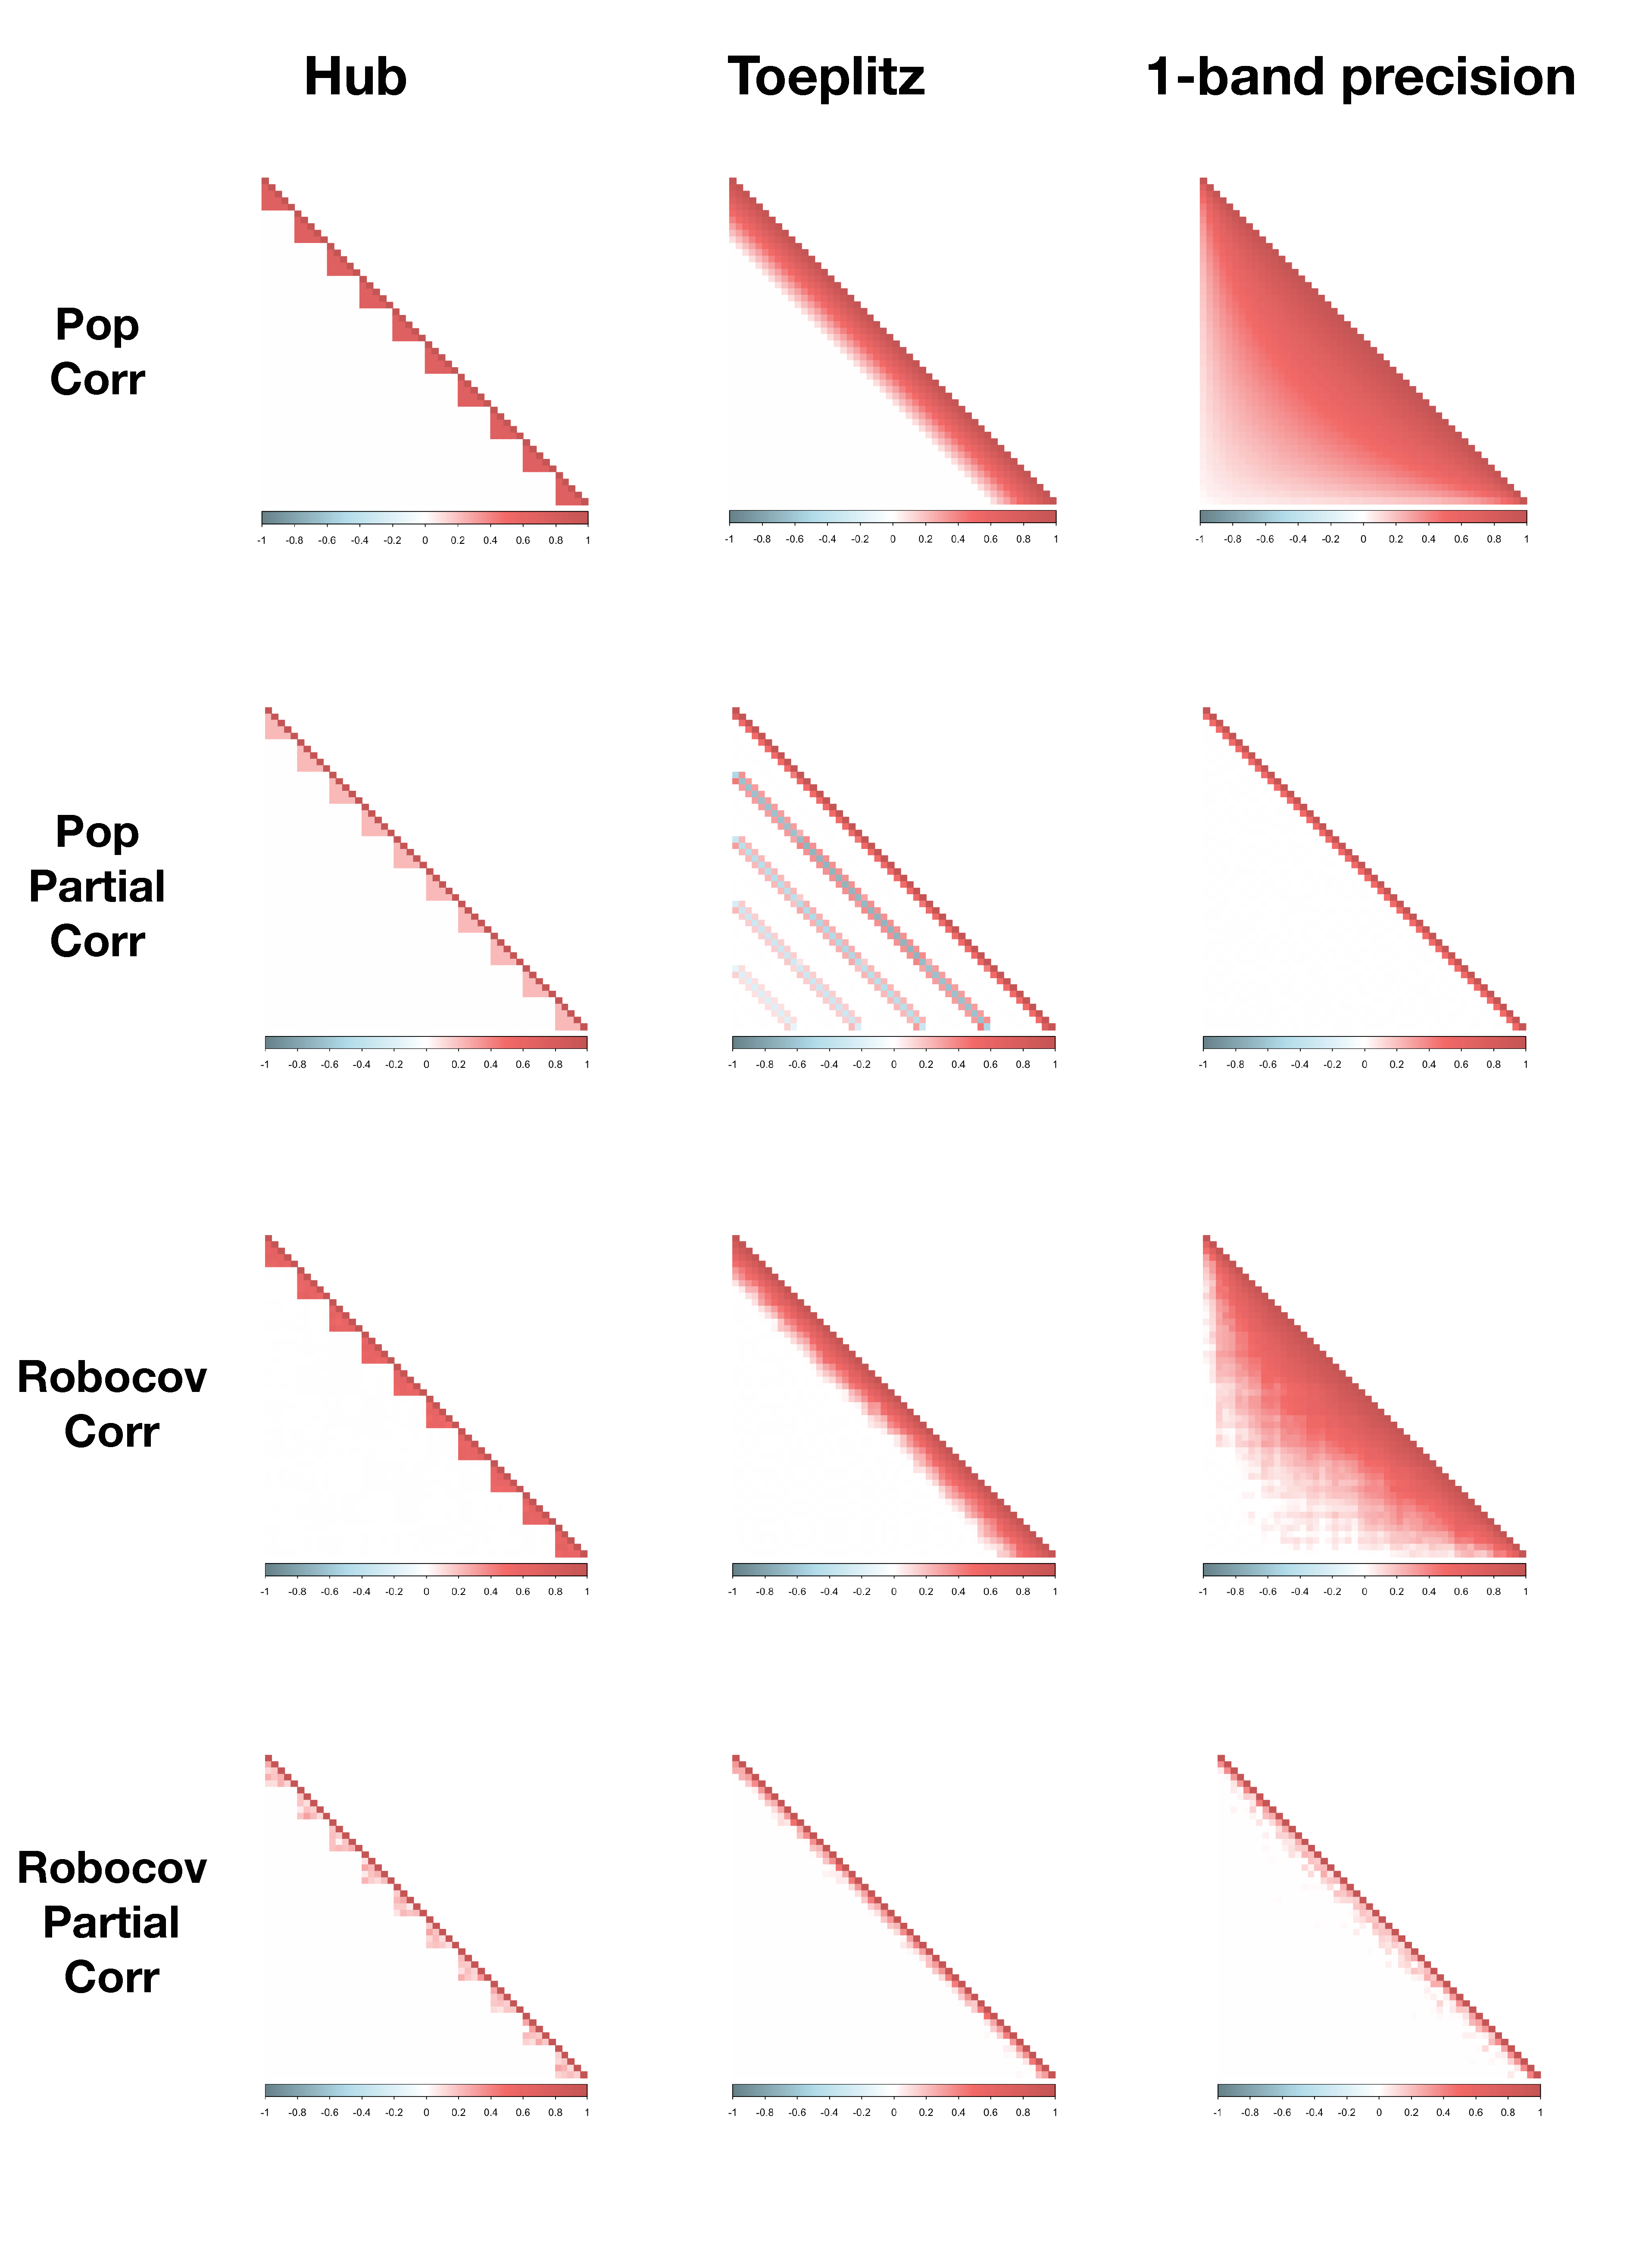
\includegraphics[width=0.5\textwidth,  trim = 0cm 5cm 0cm 0cm, clip = true  ]{Figure1_eps.eps}}
\caption{We applied \Robocov{} correlation and partial correlation estimators on data generated from Hub, Toeplitz or 1-band precision matrix based population models (Supplementary Note) with $N=500$ samples, $P=50$ features and $\pi=0.5$ proportion of missing data. We present the population correlation matrix, population partial correlation matrix, \Robocov{} correlation matrix and \Robocov{} partial correlation matrix sequentially from first to last row.}
\label{fig:sim_results}
\end{figure}

Recent work~\cite{dey2019} has shown hub-like patterns in expression correlation across tissue pairs for most genes. To this end, we applied \Robocov{} on simulated data for hub population correlation matrix structure for different settings of $N$, $P$ and $\pi$ (Supplementary Note). Two metrics of particular interest were the false positive rate (FPR) and the false negative rate (FNR) (Supplementary Note). We used these metrics to compare \Robocov{} correlation estimator with both the pairwise sample correlation estimator and  \CorShrink{}\cite{dey2019}. Across different ($N, P$, $\pi$)-settings, the \Robocov{} correlation estimator had lower FPR than \CorShrink{}. In comparison, for data with a large number of missing entries (i.e., high $\pi$), FNR for \Robocov{} was worse compared to \CorShrink{} (Table \ref{tab:tab1}). We did not compare against other shrinkage-based correlation estimators such as \textit{PDSCE}\cite{rothman2012} and \textit{corpcor}\cite{schafer2004empirical, schafer2005shrinkage} as (i) they do not account for missing entries in the data and have been shown to be sub-optimal to  \CorShrink{} for fully observed data (see Figure 4 from ref.\cite{dey2019}). 

%against estimators available from GLASSO and CLIME. Data is generated from a hub-structured population covariance matrix with different choices of $N$, $P$ and $\pi$. The three metrics are FP2 (False Positive 2-norm), FPR (False Positive Rate) and FNR (False Negative Rate). See Supplementary Note for the details of the metrics. Results are averaged over 50 replications from the same model. For all three partial correlation estimators:  \Robocov{} partial correlation, GLASSO and CLIME; the optimal sparsity inducing parameter $\lambda$ was chosen by cross-validation


\small
\begin{table}[h]
\caption{{We compare three metrics: FP2 (False Positive 2-norm), FPR (False Positive Rate) and FNR (False Negative Rate) (Supplementary Note) to compare (i) the  \Robocov{} correlation estimator (\textit{Cor}) against \CorShrink{} and the standard pairwise sample correlation estimator; and (ii) the \Robocov{} partial correlation estimator (\textit{PCor})  against estimators available from GLASSO and CLIME. Data was generated for different (N, P, $\pi$) settings and results were averaged over 50 replications from same model. Optimal $\lambda$ was chosen by cross-validation.}}
\label{tab:tab1} 
\begin{tabular}[!t]{|p{0.5cm}|p{1.1cm}|p{0.4cm}|p{0.45cm}|p{0.45cm}|p{0.4cm}|p{0.45cm}|p{0.45cm}|p{0.4cm}|p{0.45cm}|p{0.45cm}|}
\hline 
\multicolumn{11}{|c|}{Hub: N = 50, P=50} \\ \hline
& & \multicolumn{3}{c|}{$\pi$=0} & \multicolumn{3}{c|}{$\pi$=0.25} & \multicolumn{3}{c|}{$\pi$=0.5} \\ \hline
 Type & Method & FP2 & FPR & FNR &  FP2 & FPR & FNR & FP2 & FPR & FNR \\ \hline 
\multirow{ 3}{*}{Cor} & \textcolor{red}{Robocov} & 0.05 &   0 &   0  & 0.14 &   0 & 0.14 & 0.26 &   0 & 0.19 \\
& \textcolor{red}{CorShrink} & 1.4 & 0.01 &  0 & 2.2 & 0.04 & 0.03 &  4 & 0.07 & 0.09 \\
& \textcolor{red}{Standard} & 6.7 & 0.24 &  0  & 8.8 & 0.30 &  0 &  15 & 0.28 & 0 \\  \hline 
\multirow{ 3}{*}{PCor} & \textcolor{blue}{Robocov} & 0.08 & 0 & 0.07 & 0.27 & 0.01 & 0.13 & 0.47 & 0 & 0.09 \\
& \textcolor{blue}{GLASSO} & 0.12 & 0 & 0.15 & 0.29 & 0.01 & 0.15 & 0.59 & 0.02 & 0.12 \\
& \textcolor{blue}{CLIME} & 1.5 & 0.09 & 0.07 & 1.4 & 0.07 & 0.08 & 1.3 & 0.08 & 0.07 \\ \hline 
\multicolumn{11}{|c|}{Hub: N = 100, P=50} \\ \hline
& & \multicolumn{3}{c|}{$\pi$=0} & \multicolumn{3}{c|}{$\pi$=0.25} & \multicolumn{3}{c|}{$\pi$=0.5} \\ \hline
Type & Method & FP2 & FPR & FNR &  FP2 & FPR & FNR & FP2 & FPR & FNR \\ \hline
\multirow{ 3}{*}{Cor} & \textcolor{red}{Robocov} & 0.05 &   0 &   0 & 0.06 &   0 &   0 & 0.18 &   0 & 0.15\\
& \textcolor{red}{CorShrink} & 0.9 &   0 &   0 & 1.3 & 0.02 &   0 & 2.9 & 0.03 & 0.01 \\
& \textcolor{red}{Standard} & 4.8 & 0.17 &   0 & 6.2 & 0.20 &  0 &  10 & 0.31 &  0 \\ \hline 
\multirow{ 3}{*}{PCor} & \textcolor{blue}{Robocov} & 0.23 & 0 & 0.06 & 0.21 & 0 & 0.09 & 0.18 & 0.03 & 0.11 \\
& \textcolor{blue}{GLASSO} & 0.11 & 0 & 0.16 & 0.23 & 0 & 0.22 & 0.29 & 0.01 & 0.24 \\
& \textcolor{blue}{CLIME}  & 1.8 & 0.12 & 0.08 & 1.8 & 0.14 & 0.09  & 1.8 & 0.16 & 0.11 \\ \hline 
\multicolumn{11}{|c|}{Hub: N = 500, P=50} \\ \hline
& & \multicolumn{3}{c|}{$\pi$=0} & \multicolumn{3}{c|}{$\pi$=0.25} & \multicolumn{3}{c|}{$\pi$=0.5} \\ \hline
Type & Method & FP2 & FPR & FNR &  FP2 & FPR & FNR & FP2 & FPR & FNR \\ \hline
\multirow{ 3}{*}{Cor} & \textcolor{red}{Robocov}  & 0.03 &   0 &   0 & 0.01 &   0 &   0 & 0.08 &   0 &   0  \\
& \textcolor{red}{CorShrink} & 0.21 &   0 &   0 & 0.32 &   0 &   0 & 0.83 &   0 &   0\\
& \textcolor{red}{Standard} & 2.1 & 0.01 &   0 & 2.8 & 0.05 &   0 & 4.4 & 0.14 &   0 \\ \hline 
\multirow{ 3}{*}{PCor} & \textcolor{blue}{Robocov} & 0.12 & 0 & 0.11 & 0.16 & 0 & 0.12 & 0.11 & 0 & 0.14 \\
& \textcolor{blue}{GLASSO} & 0.16 & 0 & 0.19 & 0.29 & 0 & 0.20 & 0.19 & 0.02 & 0.20 \\
& \textcolor{blue}{CLIME} & 2.1 & 0.11 & 0.16 & 2.0 & 0.14 & 0.18 & 2.0 & 0.15 & 0.17 \\ \hline
\end{tabular}
\end{table}
 
\normalsize
Next, we assess the performance of the \Robocov{} partial correlation estimator for the same simulation settings (Table \ref{tab:tab1}). We are not aware of a sparse conditional graph or partial correlation estimation method that directly takes into account missing entries. Nevertheless, we compare the \Robocov{} partial correlation estimator with (i) GLASSO on the pairwise sample correlation estimator $\hat{\Sigma}$ and (ii) CLIME on an imputed data matrix where, the imputation is performed using SoftImpute~\cite{mazumder2015}. In the presence of missing data, \Robocov{} partial correlation estimator showed better FPR and FNR compared to both GLASSO and CLIME-based estimators (Table \ref{tab:tab1}). The underperformance of CLIME may be attributed to the error arising from the imputation step (Table \ref{tab:tab1}).


Next, we evaluate the predictive performance of \Robocov{} correlation estimator with pairwise sample correlation estimator and \CorShrink{}. We considered the GTEx gene expression data for an example gene (ARHGAP30) across 544 donors and 53 tissues with close to $70 \%$ missing data owing to subjects contributing only a small fraction of tissues. We split the individual by tissue data for the gene into two equal groups and  compared the estimated correlation matrix (we used different estimators: \Robocov{}, \CorShrink{} and pairwise sample correlation matrix) computed on one half of the individuals with the pairwise sample correlation matrix computed from the other half.  Both \Robocov{} and \CorShrink{} estimators considerably outperformed the pairwise sample correlation estimator, with \CorShrink{} having slightly better predictive accuracy (Figure \ref{fig:gtex_predictive} and Table \ref{tab:gtex_predictive}). As \Robocov{} and \CorShrink{} predictive performances are similar, the former may be preferable 
%in terms of interpretability.
as it results in sparse estimates, leading to better interpretability. 


An an alternative to \Robocov{}, we may consider an estimator obtained by first imputing the missing entries in the data matrix and then estimating the correlation or partial correlation matrix for the complete data. For the same ARHGAP30 gene, we performed imputation by either a low rank factorization (SoftImpute\cite{mazumder2015}, with or without scaling) or a median based approach (replacing the missing entries of a feature by the median value of the observed entries). The correlation matrix obtained by SoftImpute (both  with and without scaling) showed artificial high negative and positive correlation sweeps between brain and non-brain tissues that were not observed in the pairwise correlation matrix (Figure \ref{fig:supp_imputed}). One possible explanation of this is that the data matrices in our case do not seem to have a low rank representation based on eigenvalue analysis (Figure \ref{fig:gtex_highrank}).  The median based imputation method on the other hand, is prone to showing false positives---for example, we see a high correlation between Fallopian tube and Cervix-Ectocervix, which is a consequence of only 3 individuals contributing  both the tissues (Figure \ref{fig:supp_imputed}). \Robocov{} can effectively get rid of these edge cases and generate sparser and more robust results compared to these imputation based approaches.

%Based on our simulation studies, we conclude that the \Robocov{} correlation estimator has a lower FPR than both the standard pairwise sample correlation estimator and \CorShrink{}. In terms of predictive performance, \Robocov{} does better than the standard estimator and is comparable to  \CorShrink{}. We also observe that for data with a large number of missing entries and no obvious low rank representation as in case of the GTEx gene expression data, imputation based approaches are sub-optimal and \Robocov{} would be the preferred option in such a scenario. The \Robocov{} partial correlation estimator, on the other hand, showed better performance both in terms of FPR and FNR compared to other competing methods such as GLASSO and CLIME, especially when the proportion of missing entries in the data matrix is high. 



%%%when there are missing entries in the data than competing approaches.


\subsection*{Gene Expression correlation analysis across tissue pairs}

\begin{figure*}[!tpb]
\centering
\scalebox{1}{\includegraphics[height=0.7\textheight]{Figure1a_eps.eps}}
\caption{\small {{Illustrative examples of pairwise sample correlation estimator, \Robocov{} correlation and partial correlation estimators for 2 genes}:
(Left column)  \textbf{ARHGAP30} gene and (Right column) \textbf{GSTM1} gene. Each column shows the (A) pairwise sample correlation estimator, (B) \Robocov{} correlation estimator and  (C) partial correlation estimator stacked from top to bottom.}}
\label{fig:gtex_demo}
\end{figure*}


We applied \Robocov{} to each of 16,069 cis-genes (genes with at least one significant cis-eQTL) from the GTEx v6 project \cite{dey2017} (see URLs). For each gene, the data matrix had 544 rows (post-mortem donors), 53 columns (tissues) and comprised of $\sim70\%$ missing entries.  Figure \ref{fig:gtex_demo} presents a visual comparison of \Robocov{} correlation and partial correlation estimators with standard pairwise sample correlation matrix for two example genes (ARHGAP30 and GSTM1)---the \Robocov{} estimators are sparse and visually less cluttered than the standard approach. The \Robocov{} correlation structure across tissue pairs varied from one gene to another: some genes showed high correlation across all tissues (e.g. HBB, RPL9), some showed little to no correlation across tissues (e.g. NCCRP1), some showed high intra-Brain correlation but relatively low inter-Brain correlation (e.g. ARHGAP30) (Figures \ref{fig:gtex_examples_main},  \ref{fig:suppfig_gtex_examples} and  \ref{fig:gtex_predictive}). Additionally, two genes with similar correlation profiles may have very distinct expression profiles. For example,  HBB and RPL9 both showed high correlation across all tissue pairs, but they had very  distinct tissue-specific expression profiles. HBB showed high expression in Whole Blood relative to other tissues, while RPL9 had a more uniform expression profile across tissues (Figure \ref{fig:gtex_examples_main}). A similar pattern was observed also for two genes with negligible correlation across tissues, NCCRP1 and RPL21P11 (Figure \ref{fig:suppfig_gtex_examples}). 



\begin{figure*}[!tpb]
\centering
\scalebox{1}{\includegraphics[height=0.7\textheight]{Figure2_eps.eps}}
\caption{\small {{Examples of genes with high average \Robocov{} correlation across all tissue pairs but with distinct expression profiles. (A)\textbf{RPL9} gene has uniformly high TPM (transcripts per million) values across most tissues (inset picture). (B) \textbf{HBB} shows high expression specifically in Whole Blood (inset picture). The expression profile plots for the genes have been fetched from the GTEx Portal (\url{https://gtexportal.org/home/}).}}}
\label{fig:gtex_examples_main}
\end{figure*}



%A general perception is that genes with high correlation in gene expression  across individuals for all tissue-pairs would be enriched for genes with uniform expression across tissues such as the housekeeping genes. Interestingly, our results in Figure \ref{fig:gtex_examples_main}, seem to suggest otherwise. 
%%evidence against
%%this perception.


Next, we assign to each gene, a prioritizing score defined by the average value of \Robocov{} correlation (\textit{Robospan-score}) or partial correlation (\textit{pRobospan-score}) across all tissue pairs. Similarly, we also computed the average value of the pairwise sample correlation (\textit{Corspan-score}) across tissues. Then we tested these gene scores for functional relevance. Contrary to expectation, none of the three scores showed significant enrichment in 3,804 housekeeping genes\cite{eisenberg2013} (0.84x, 0.48x and 0.72x for Robospan-score,  pRobospan-score and Corspan-score  respectively). We compared these 3 gene scores with constraint-based metric of gene essentiality such as the absence of loss-of-function(LoF) variants (pLI\cite{Lek2016} and s\_het\cite{cassa2017}). For each of the 50 quantile bins of pLI and s\_het, we computed the median of each of these scores; and compared with the mid-value of the quantile bin. We observed a slight negative trend in all 3 scores with increasing quantile bins of both pLI and  s\_het  (Figure \ref{fig:pLI_shet}). One possible explanation may be that genes with highly correlated expression across all tissues may be driven by tissue-shared regulation machinery which imposes lower selective constraints on these genes. 
The top 10$\%$ genes from each of the three gene prioritizing scores were used to define gene sets; we call them \Robospan{}, \pRobospan{} and \Corspan{} genes. In a pathway  enrichment analysis\cite{Kamburov2012} of these gene sets, the top enriched pathways comprised of immune system, interferon signaling, heat stress factor (Table \ref{tab:pathway}). Though not among the top 5 pathways, other interesting significant pathways included different signaling pathways (interleukin mediated signaling, NFkB signaling) and circadian clock related pathways (see URLs). The signifcance of pathway enrichment was stronger for \Robospan{} and \pRobospan{} genes compared to \Corspan{}(Table \ref{tab:pathway}). The enrichment of immune related pathways was further backed by high enrichment of these genes in top 10$\%$ specifically expressed genes in Whole Blood (SEG-Blood\cite{Finucane2018}) (\Robospan{}: 1.48x, \pRobospan{}: 2.50x, \Corspan{}: 1.45x). One may conjecture that this enrichment is an artifact caused by contamination of blood with GTEx tissue samples. This, however, is countered by examples of genes that have high correlation across all tissues but expression-wise, are specific to tissues that are not Whole Blood (Figure \ref{fig:suppfig_gtex_examples_2}). We also see examples of specifically expressed genes in Whole Blood that have low Robospan-score (Figure \ref{fig:suppfig_gtex_examples_3}).

\subsection*{Heritability analysis of blood-related traits}

%We conclude that \Robocov{} produces less visually cluttered representation of correlation and partial correlation structure of gene expression across tissue pairs for individual genes. We also show that genes with high average \Robocov{} correlation or partial correlation across tissue pairs tend to have lower selection constraint and are not enriched for housekeeping genes. The top genes with highest average \Robocov{} correlation or partial correlation across tissues are enriched for immune related functionality among other systemic pathways such as heat stress factors, circadian clock etc. This is further backed by enrichment of \Robospan{} and \pRobospan{} genes with specifically expressed genes in Blood. 
The enrichment of \Robospan{}, \pRobospan{} and \Corspan{} genes with SEG-Blood genes and immune related pathways prompted us to test whether these genes are uniquely informative for blood-related complex diseases and traits.

\begin{figure}[!tpb]
\centering
\scalebox{1}{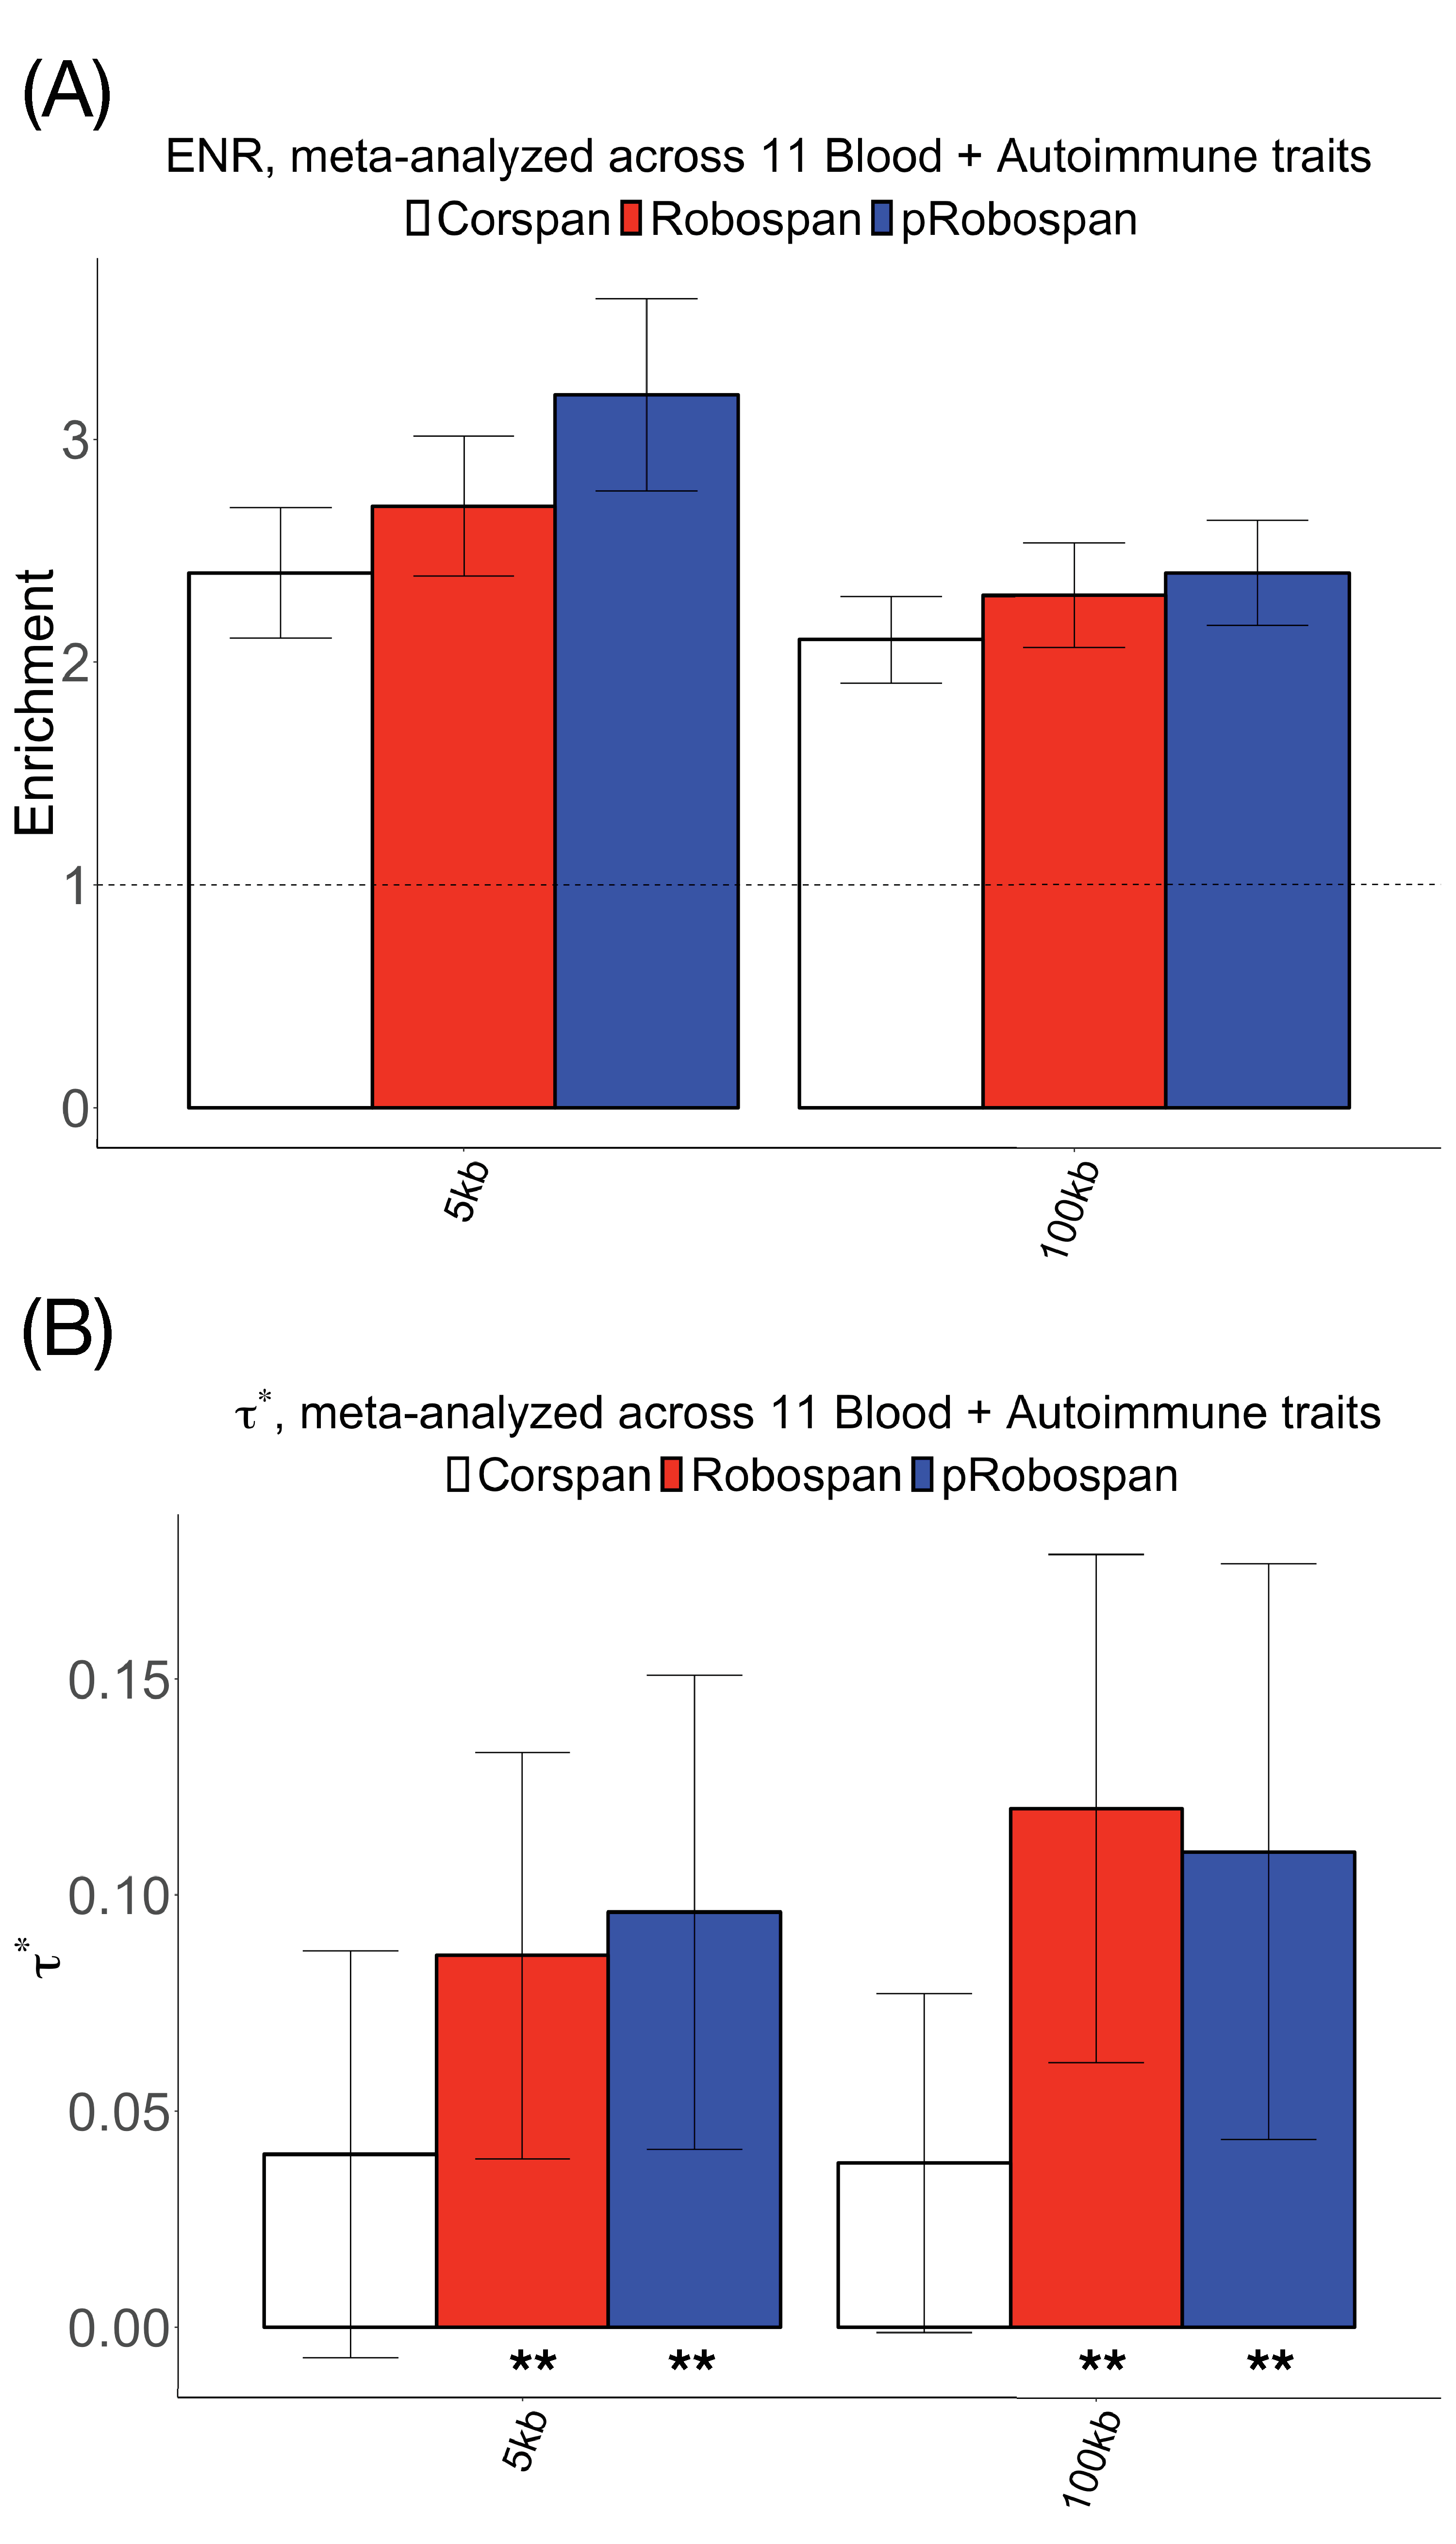
\includegraphics[width=0.4\textwidth]{Figure3_eps.eps}}
\caption{\small {\textbf{Disease informativeness of 5kb and 100kb SNP annotations for \Corspan{}, \Robospan{} and \pRobospan{} gene sets}: (A) Heritability enrichment, conditional on baseline-LD model (v2.1). The base enrichment level is 1. (B) Standardized effect size ($\tau^{\star}$) conditional on baseline-LD model for \Corspan{} (left column, white), \Robospan{} (middle column, red) and \pRobospan{} (right column, blue) gene sets. Results are meta-analyzed across 11 blood and autoimmune traits. ** denotes annotations that are significant after Bonferonni correction ($P < 0.05/8$) where $8$ is the total number of SNP annotations tested. Error bars denote 95$\%$ confidence intervals. Numerical results are reported in Table \ref{tab:Robocov_marginal}.}}
\label{fig:Robocov_marginal}
\end{figure}

For each gene set, we define  SNP-level annotations to test for disease heritability. We define an \emph{annotation} as an assignment of a numeric value to each SNP with minor allele count $\geq$5 in a 1000 Genomes Project European reference panel\cite{1000G2015, Finucane2015}. For each gene set X, we generate two binary SNP-level annotations -- we assign a value of 1 to a SNP if it lies within 5kb or 100kb window upstream and downstream of a gene in the gene set and 0 otherwise; this strategy has been used in several previous works\cite{Finucane2018, Kim2019, deLeeuw2015}.

We assessed the informativeness of SNP annotations for disease heritability by applying stratified LD score regression (S-LDSC)\cite{Finucane2015} conditional on 86 baseline annotations comprising of coding, conserved, epigenomic and LD related annotations (this is called the baseline-LD model; here we use version 2.1\cite{gazal2017}). S-LDSC results were meta-analyzed across 11 relatively independent blood-related traits (5 autoimmune diseases and 6 blood traits (Table \ref{tab:list_blood_traits}).  We considered two S-LDSC metrics for comparison: enrichment and standardized effect size ($\tau^{\star}$) (Supplementary Note).  Enrichment is defined as the proportion of heritability explained by SNPs in an annotation divided by the proportion of SNPs in the annotation\cite{Finucane2015}. Standardized effect size ($\tau^{\star}$) is defined as the proportionate change in per-SNP heritability associated with a 1 standard deviation increase in the value of the annotation, conditional on other annotations included in the model\cite{gazal2017, Hormozdiari2018}; unlike enrichment, $\tau^{\star}$ quantifies effects that are unique to the focal annotation and is a better metric for disease informativeness\cite{dey2019, Kim2019, Finucane2018, Hormozdiari2018}. 

%In our ``marginal'' analyses, we estimated $\tau^{\star}$ for each focal annotation conditional on the 90 baseline-LD$^\star$ annotations. 

All $6$ annotations (5kb and 100kb for the 3 gene scores) were significantly enriched when meta-analyzed across 11 blood and autoimmune traits. However, SNP annotations corresponding to \Robospan{} and \pRobospan{} gene sets showed higher enrichment than  \Corspan{} genes (Figure \ref{fig:Robocov_marginal} and Table \ref{tab:Robocov_marginal}). More importantly, 2 \Robospan{}, 2 \pRobospan{} and 0 \Corspan{} annotations showed significant $\tau^{\star}$ conditional on the baseline-LD annotations after Bonferonni correction (Figure \ref{fig:Robocov_marginal} and Table \ref{tab:Robocov_marginal}). When restricted to the 5 autoimmune traits,  2 \Robospan{}, 0 \pRobospan{} and 0 \Corspan{} SNP annotations showed unique signal (Table \ref{tab:Robocov_marginal_immune}). Even when these annotations were modeled jointly with SEG-Blood\cite{Finucane2018} genes and subjected to forward stepwise elimination similar to ref.\cite{Kim2019, dey2019}, 1 \Robospan{} annotation (100kb) still remains significantly informative, suggesting unique disease information over SEG-Blood genes (Table \ref{tab:Robocov_joint}). 

%obocov{} correlation and partial correlation estimator show higher enrichment and disease informative signal compared to the \Corspan{} gene set constructed similarly from the standard correlation estimator. Additionally, the \Robospan{} gene set shows unique disease information ($\tau^{\star}$) conditional on the specifically expressed gene in blood; this shows that the study of correlation structure of gene expression across tissues adds value over study of expression data alone. 






















\section{Discussion}\label{sec:discussion}

Here we present \Robocov{}---a novel convex optimization-based framework for sparse estimation of covariance (correlation) and inverse covariance (partial correlation) matrix, given a data matrix with missing entries. Our approach does not rely on missing data imputation and hence mitigates the possible shortcomings of a sub-optimal imputation procedure (e.g., based on a low-rank assumption). Instead, \Robocov{} directly estimates the correlation or partial correlation matrix of interest via a regularized loss minimization framework. Although here we focus our analysis on gene expression analysis, \Robocov{} is a stand-alone generic tool that can be applied to any data with missing entries.
%when the data matrix contains missing entries and does not allow a low rank representation to enable accurate imputation. 

We have assessed the significance of our proposed \Robocov{} framework over standard methods from a methodological, biological and disease analysis perspective. \Robocov{} leads to sparse estimates and has a lower false positive rate compared to other competing methods. \Robocov{} estimator is visually less cluttered and captures more robust biological signal. In terms of disease informativeness, \Robospan{} and \pRobospan{} gene sets, generated from the \Robocov{} estimated correlation and partial correlation matrices, perform considerably better than the analogous \Corspan{} gene set defined from standard correlation estimator.  

%\Robocov{} also provides better disease signal than the standard approach --- \Robospan{} and \pRobospan{} gene sets are more informative for blood and autoimmune traits over \Corspan{} gene set. 

%Our method has several limitations that can motivate future research directions. First, \Robocov{} assumes that all missing entries in the data matrix are missing at random. 
There are several directions for future research. One such direction would be to incorporate covariate information underlying structured missing-ness to inform \Robocov{} estimators. For GTEx data, donor metadata such as cause of death, age, gender etc can serve as important covariates.  Second, we are interested in modifying \Robocov{} to learn shared correlation structure between gene expression and other genetic and epigenomic data such as transcript level expression, ATAc-seq data etc. Third, from application standpoint, \Robocov{} can also be used as an ingredient in item response models for large scale participant data that may contain extensive amount of missing entries, as in UK Biobank  \cite{Sulis2017, Bauermeister2019}.

\section*{URLs}
\small
\begin{itemize}
    \item \Robocov{} software \\
    \url{https://github.com/kkdey/Robocov}
    \item GTEx v6 data analysis, gene list,
    pathway enrichment results, gene sets,
    annotations\\
    \url{https://github.com/kkdey/Robocov-pages}
    \item Baseline-LD annotations:\\ 
    \url{https://data.broadinstitute.org/alkesgroup/LDSCORE/}
    \item Summary statistics:\\ 
    \url{https://data.broadinstitute.org/alkesgroup/sumstats_formatted/}
\end{itemize}

\normalsize
\section*{Acknowledgements}

We thank Alkes L. Price, Bryce van de Geijn and Rajarshi Mukherjee for helpful comments. Rahul Mazumder was partially supported by 
the Office of Naval Research ONR-N000141512342, ONR-N000141812298 (Young Investigator Award), the National Science Foundation (NSF-IIS-1718258) and IBM.





\end{document}

